\chapter{Future Works}
This section describes future work that could be conducted within the problem area. Some suggestions are related to our implementation, some are related to the research conducted using the prototype.
\section{Prototype related future works}
\textbf{Knowing where the client is in the garden, while the architect is building it.} In addition to this some kind of marker could be installed to track where the client was in the VR world and that would show op on the glass plate for the architect to know exactly where the client was at that moment. To which degree how easy or difficult this would be to install is not considered yet, but it needs to be efficient and not slowing down the system or being more cumbersome than necessary\todo{(Also rotation) Could possibly be achieved via laser pointer on motor - otherwise we'd likely need a projector system just like Steven's}.\\

\textbf{Making the prototype lighter and easier to handle}.\\
Another way to ease our prototype is to make it lighter. Basically this would be using another more transportable VR unit, that doesn't need as much setup time as it do right now. Further more another webcam would be preferred.\\
Regarding the box, it needs to be the right size for the camera used so that we don't have any parts on the glass plate where the marker wont show up in the VR world. The box itself would be made lighter and in a way that makes it easier to transport.\\

\textbf{Allow architects to draw sections on the plate, then place a marker inside them to place multiple objects, or change texture}.\\ One problem with the current implementation is that it is impossible to do things like a flowerbed. During the usability test one test person also remarked that the ability to create custom shaped pond would be nice. The idea is reasonably simple, one can draw enclosed shapes on the plate. Placing a marker inside this will cause the entire shape to be filled with the marker's object. Rotating the flower would control the density of the objects in the shape. This could also be used to add things like tiled paths, or walls to the garden, making it look way more like a real garden. How the implementation could work can be seen in Figure \ref{fig:ftemarkers}, and \ref{fig:ftrmarkerslegend}. The old markers on the top are just due to the reuse of the old model.
\begin{figure}[H]
	\centering
	\begin{minipage}[b]{0.49\textwidth}
		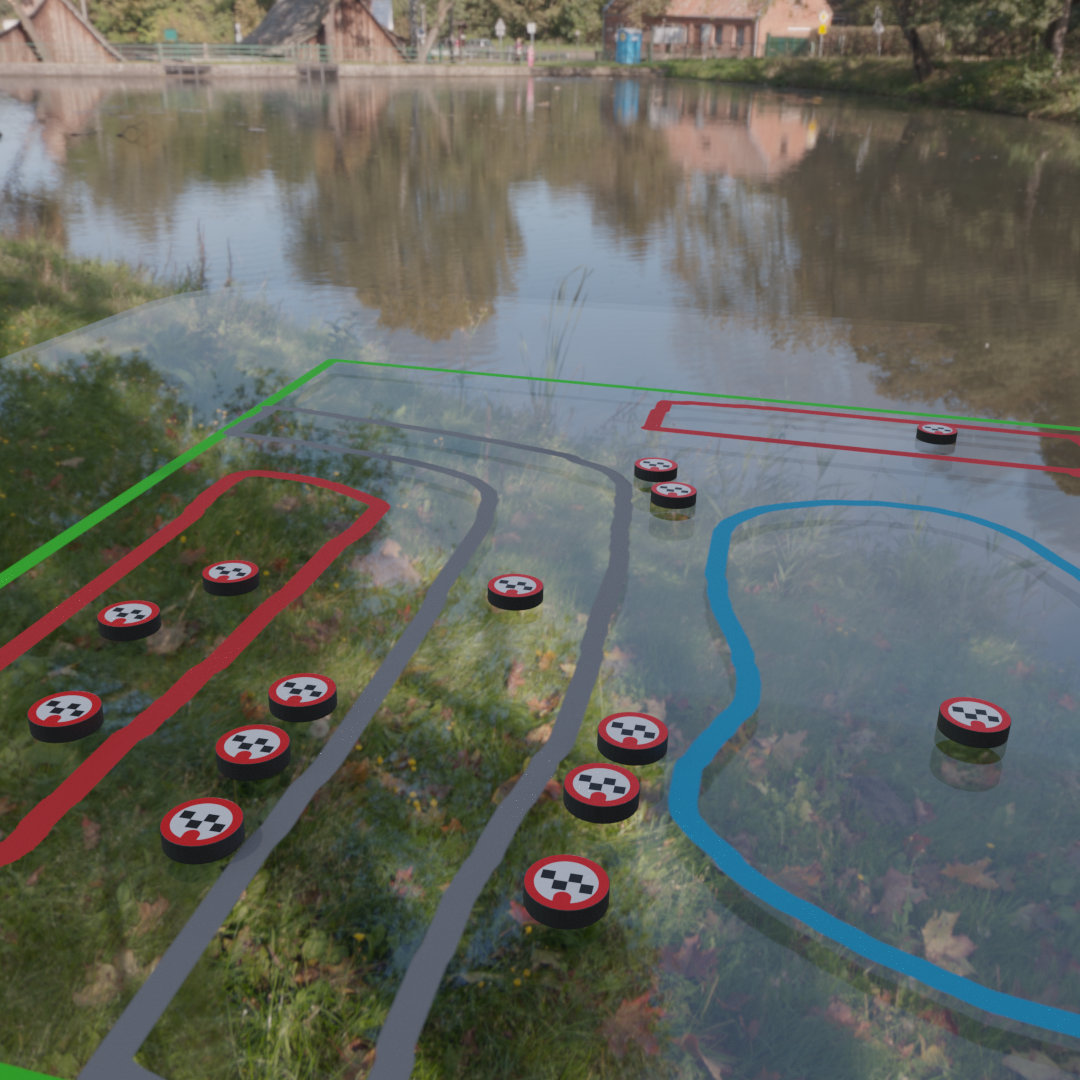
\includegraphics[width=1.0\linewidth]{figure/Evaluation/futuremarkers.png}
		\caption{Implementing this would allow architect to create flowerbeds, place multiple objects at a time, as well as change textures.}
		\label{fig:ftemarkers}
	\end{minipage}
	\hfill
	\begin{minipage}[b]{0.49\textwidth}
		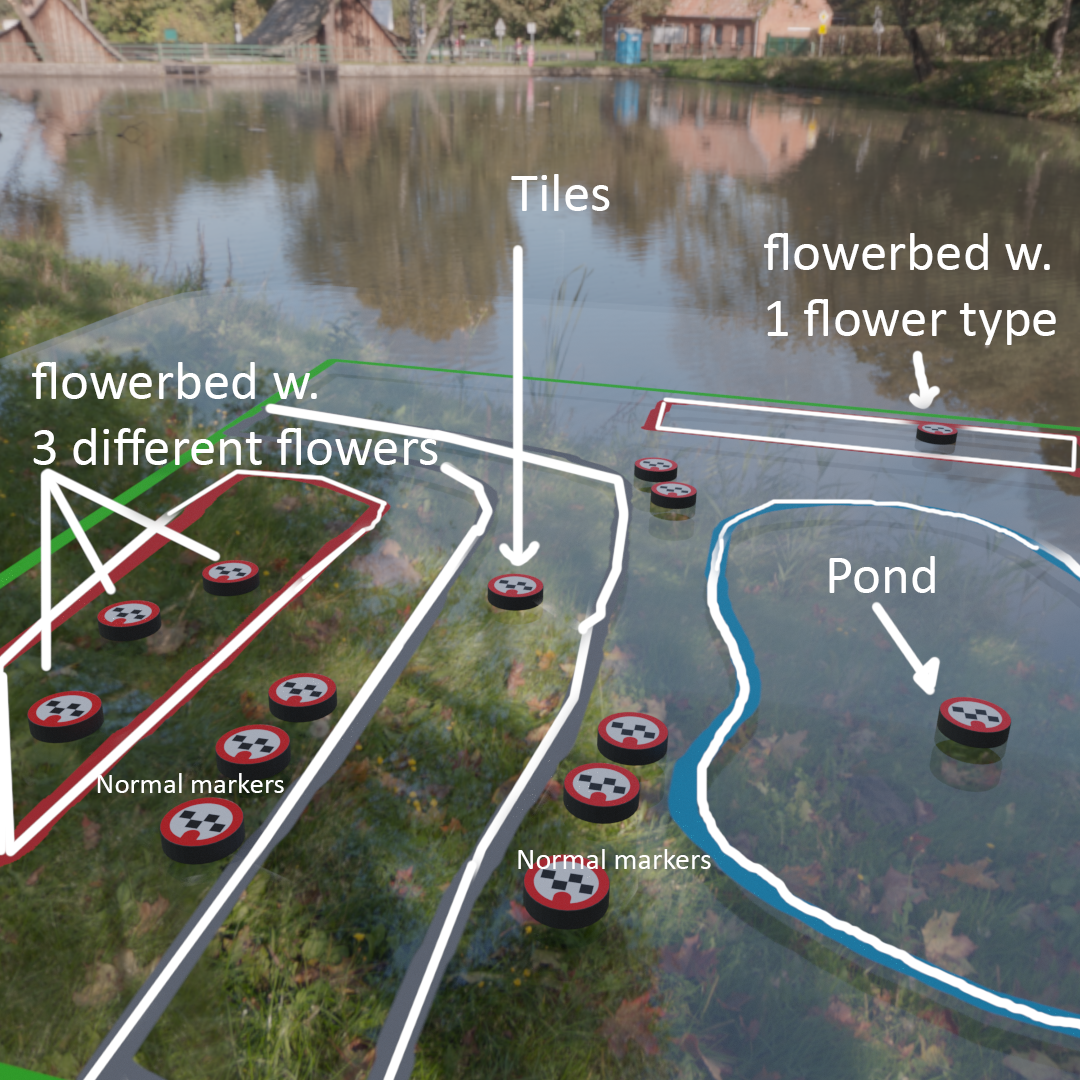
\includegraphics[width=1.0\linewidth]{figure/Evaluation/futuremarkerslegend.png}
		\caption{Explanation of what the Figure to the right would be interpreted as using this solution.}
		\label{fig:ftrmarkerslegend}
	\end{minipage}
\end{figure}

\textbf{Adding the ability to export plant lists and measurements}.\\
When the landscape architect and customer have agreed upon a final design there should to be an export functionality that gathers all the data from the tokens on the board and export plant lists and measurements etc. for the customer who can pass it on to a gardener and/or a paver as blueprints for their work.

\todo{Optimize rendering or models for better fps on low-end systems}
\todo{Consistency in object rotation (no more jittering)}
\todo{More varied kinds of objects and more of each}
\todo{Better ability for architect to see orientation and relative size of objects - a good solution would be 3d printed markers that are correctly scaled.}
\todo{Ability to change object sizes?}
\section{Evaluation related future work}

Better expert related research would be critical to establish the usefulness of the product inside the problem areas. Future researches should consider ways to get in contact garden architects to ensure testers, as they proved an illusive target group.